
\section{VI - Reconnaissance de mot}
\begin{frame}{VI - Reconnaissance de mot}
	\begin{block}{}
		Le site du gouvernement recense ces mots-clés pour les numéros d'appel d'urgence : \\
		\begin{description}
			\item[n°15] malaise, hémorragie, brûlure, intoxication
			\item[n°17] violences, agression, vol, cambriolage
			\item[n°18] incendie, gaz, effondrement, électrocution
		\end{description}
	\end{block}
	\begin{figure}
		\begin{subfigure}[]{0.3\textwidth}
			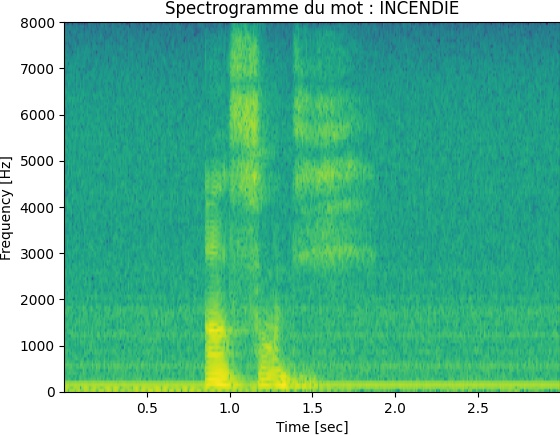
\includegraphics[width=\textwidth]{1-Incendie.jpg}
			\caption{INCENDIE}
		\end{subfigure}
		\begin{subfigure}[]{0.3\textwidth}
			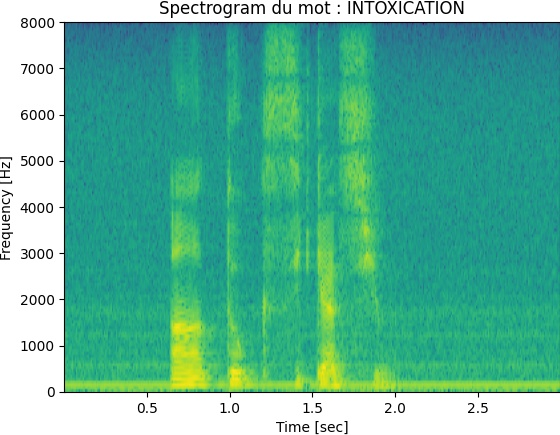
\includegraphics[width=\textwidth]{1-Intoxication.jpg}
			\caption{INTOXICATION}
		\end{subfigure}
		\begin{subfigure}[]{0.3\textwidth}
			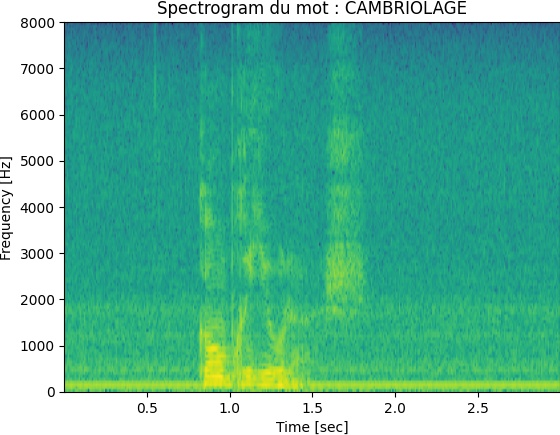
\includegraphics[width=\textwidth]{1-Cambriolage.jpg}
			\caption{CAMBRIOLAGE}
		\end{subfigure}
	\end{figure}
\end{frame}


\begin{frame}{VI - Transfert d'apprentissage}
	\begin{figure}
		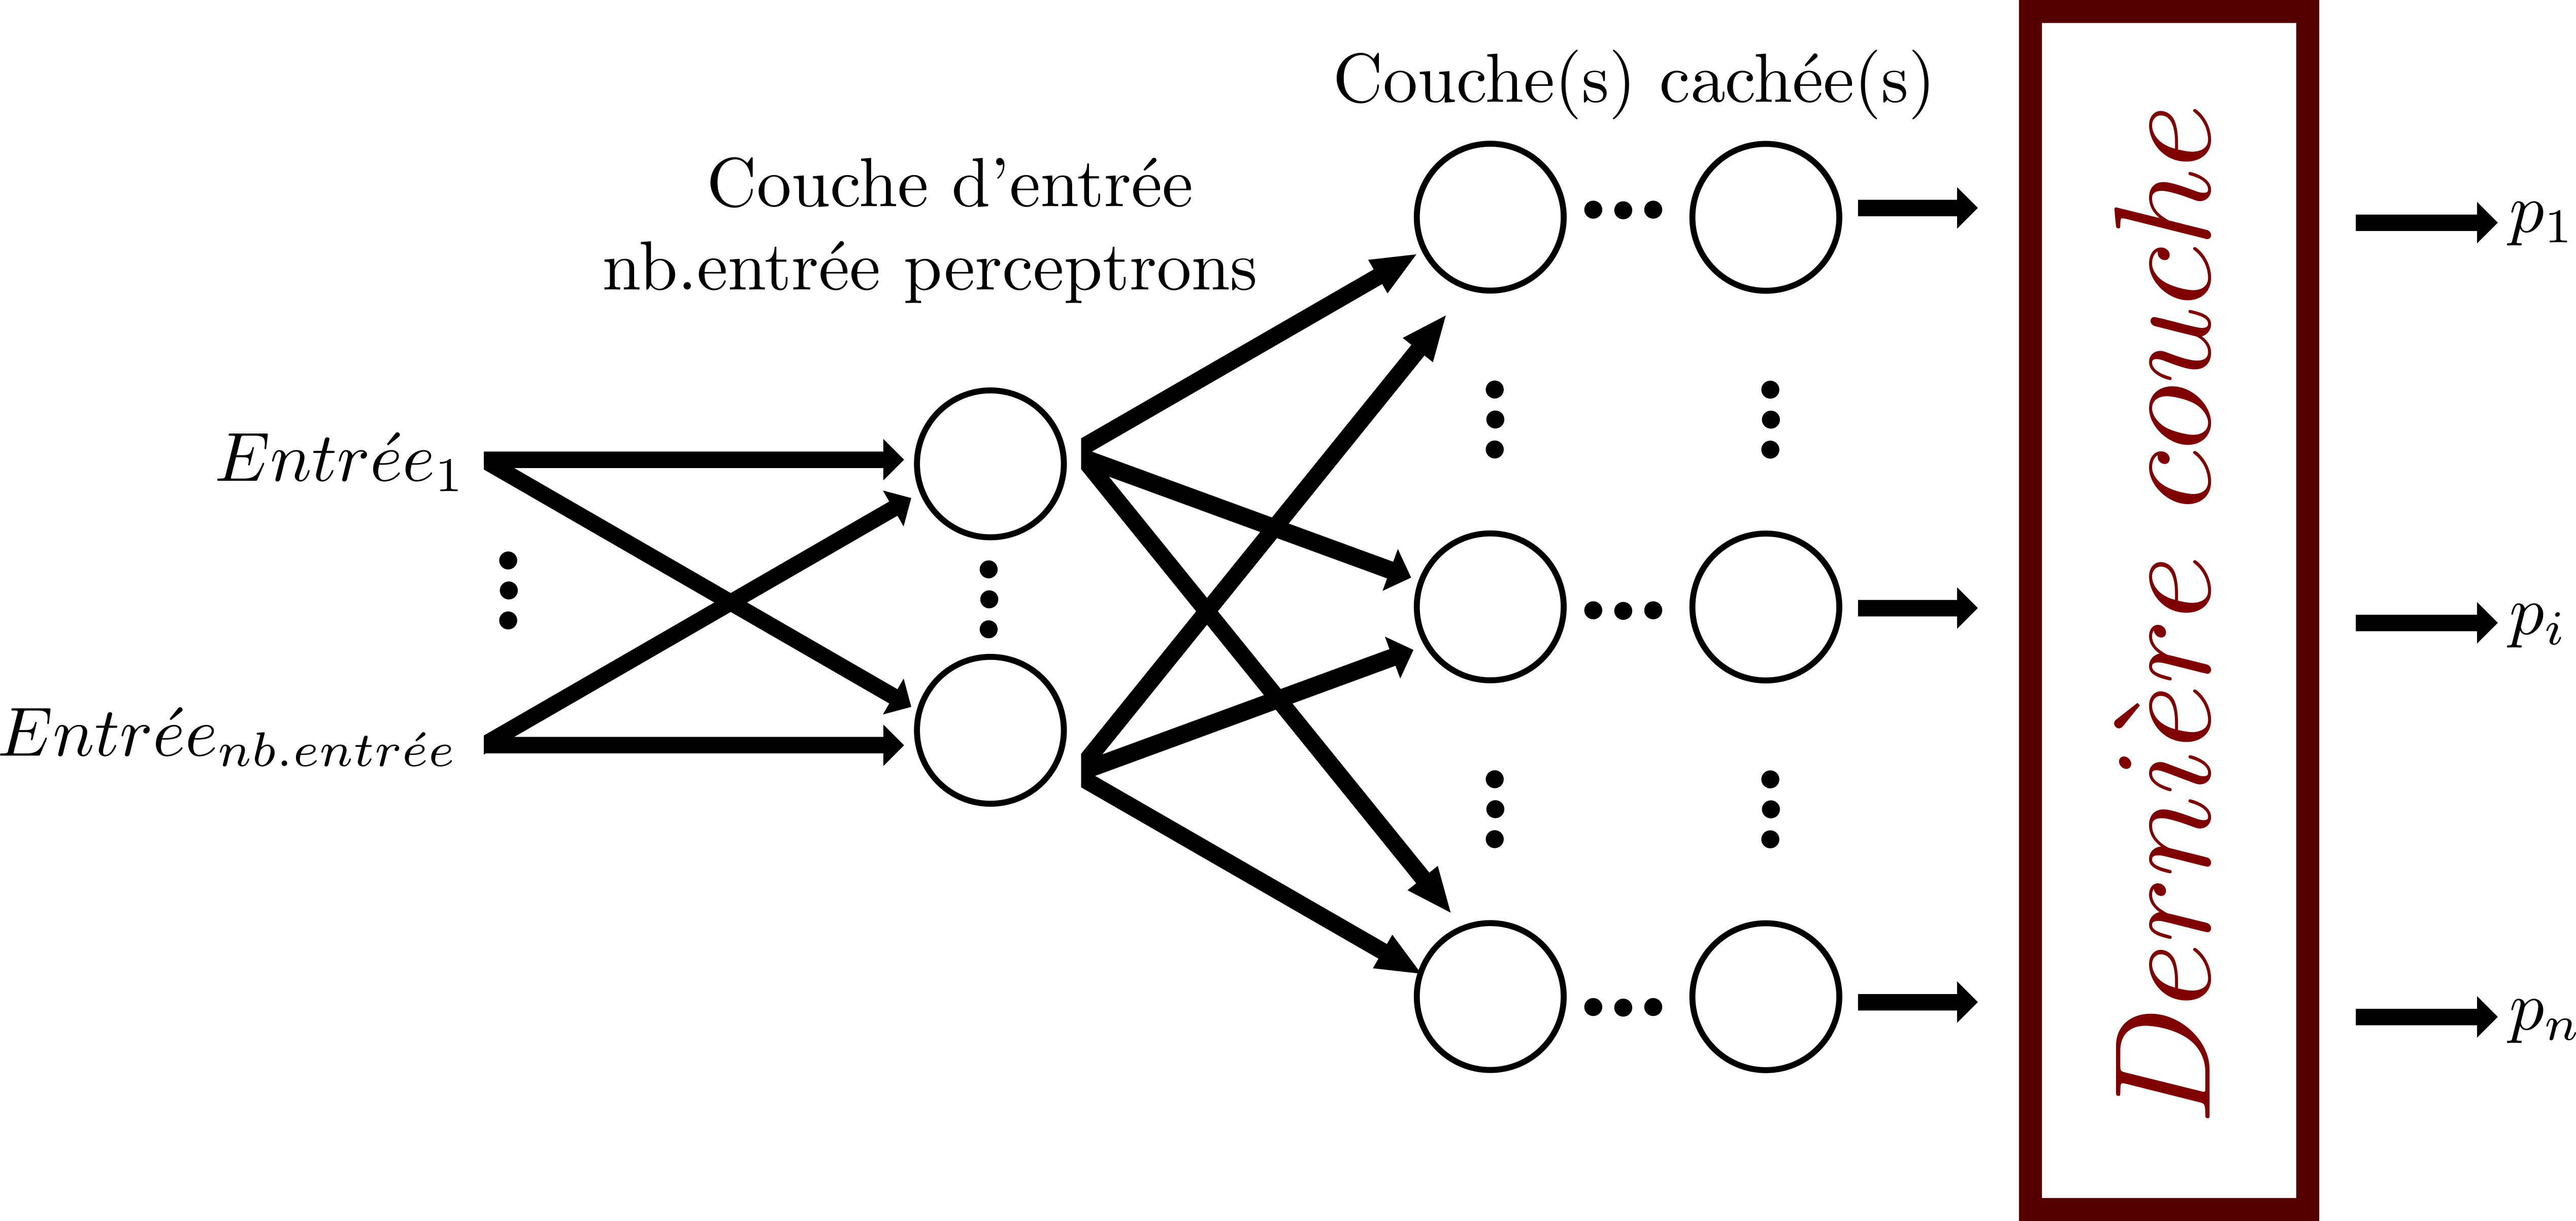
\includegraphics[width=\textwidth]{2-transfert.png}
		\caption{Schéma de fonctionnement du transfert d'apprentissage}
	\end{figure}
\end{frame}


\begin{frame}{VI - Réseau de neurones modèle}
	\lstinputlisting[]{7-model}
\end{frame}


\begin{frame}{VI - Entrainement du réseau modèle}
	\begin{block}{Modèle}
		Le réseau modèle est entrainé sur 8 000 données pour reconnaitre les $8$ mots : \\
		$["no",\ "stop",\ "up",\ "right",\ "yes",\ "left",\ "go",\ "down"]$ \\
	\end{block}
	\begin{exampleblock}{Adaptation}
		Nous voulons que notre réseau de neurones reconnaisse les $12$ mots : \\
		$["malaise", "h\acute{e}morragie", "br\hat{u}lure", "intoxication",$ \\
					$ "violences", "agression", "vol", "cambriolage",$ \\
					$ "incendie", "gaz", "effondrement", "\acute{e}lectrocution"]$
	\end{exampleblock}
	\lstinputlisting[language=Python, firstline=15]{8-transfert.py}
\end{frame}


\begin{frame}{VI - Réseau de neurones modèle}
	\lstinputlisting[]{9-model2}
\end{frame}

\begin{frame}{VI - Mes résultats}
	\begin{figure}
		\begin{subfigure}[]{0.45\textwidth}
			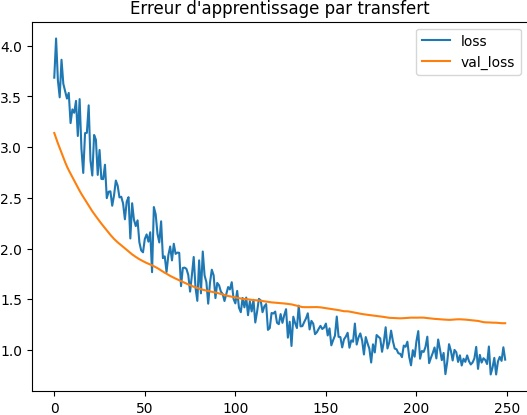
\includegraphics[width=\textwidth]{4-loss.jpg}
			\caption{Erreur au cours de l'apprentissage}
		\end{subfigure}
		\begin{subfigure}[]{0.45\textwidth}
			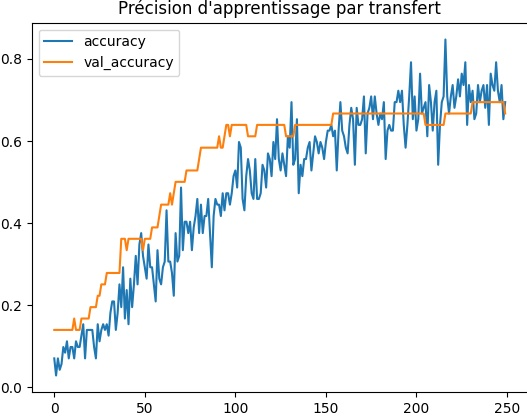
\includegraphics[width=\textwidth]{4-accuracy.jpg}
			\caption{Taux de bonnes réponses}
		\end{subfigure}
	\end{figure}
\end{frame}

\begin{frame}{VI - Analyse de mes résultats}
	\begin{columns}[T]
		\begin{column}[]{0.45\textwidth}
			\begin{exampleblock}{Données d'apprentissage}
				\begin{description}
					\item[Agathe]  $1\times12$ données
					\item[Florent]  $1\times12$ données
					\item[Tien-Thinh]  $4\times12$ données
				\end{description}
			\end{exampleblock}
		\end{column}
		\begin{column}[]{0.45\textwidth}
			\begin{alertblock}{Données d'évaluation}
				\begin{description}
					\item[Agathe]  $1\times12$ données
					\item[Florent]  $1\times12$ données
					\item[Tien-Thinh]  $1\times12$ données
				\end{description}
			\end{alertblock}
		\end{column}
	\end{columns}
	\begin{columns}[T]
		\begin{column}[]{0.45\textwidth}
			\begin{figure}
				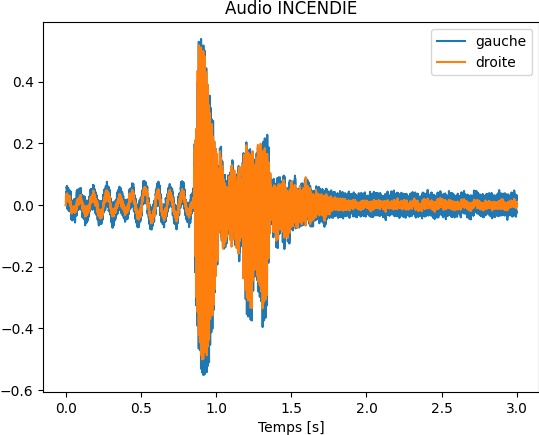
\includegraphics[width=\textwidth]{5-Audio.jpg}
			\end{figure}
		\end{column}
		\begin{column}[]{0.45\textwidth}
			\begin{block}{Précision finale}
				\begin{description}
					\item[Agathe]  $50\%$ accuracy
					\item[Florent]  $75\%$ accuracy
					\item[Tien-Thinh]  $75\%$ accuracy
				\end{description}
			\end{block}
		\end{column}
	\end{columns}
\end{frame}


\begin{frame}{VI - Analyse découpage en formant}
	\begin{block}{Formant - Définition Larousse}
		Fréquence de résonance du conduit vocal. \\
		Les voyelles se définissent acoustiquement par leurs formants; \\
		seules les consonnes dites vocaliques présentent une structure formantique similaire à celle des voyelles.
	\end{block}
	\begin{figure}
		\begin{center}
			\centering
			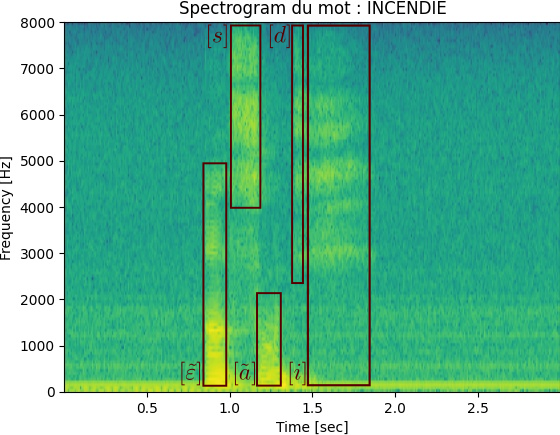
\includegraphics[width=0.45\textwidth]{3-incendie.png}
			\caption{Analyse de formant du mot "INCENDIE" \\avec l'aide de Mme.Voisin en formation d'orthophonie à la Sorbonne}
		\end{center}
	\end{figure}
\end{frame}


\begin{frame}{VI - Mon réseau de neurones reconnaissant les mots-clés}
	\begin{figure}
		\centering
		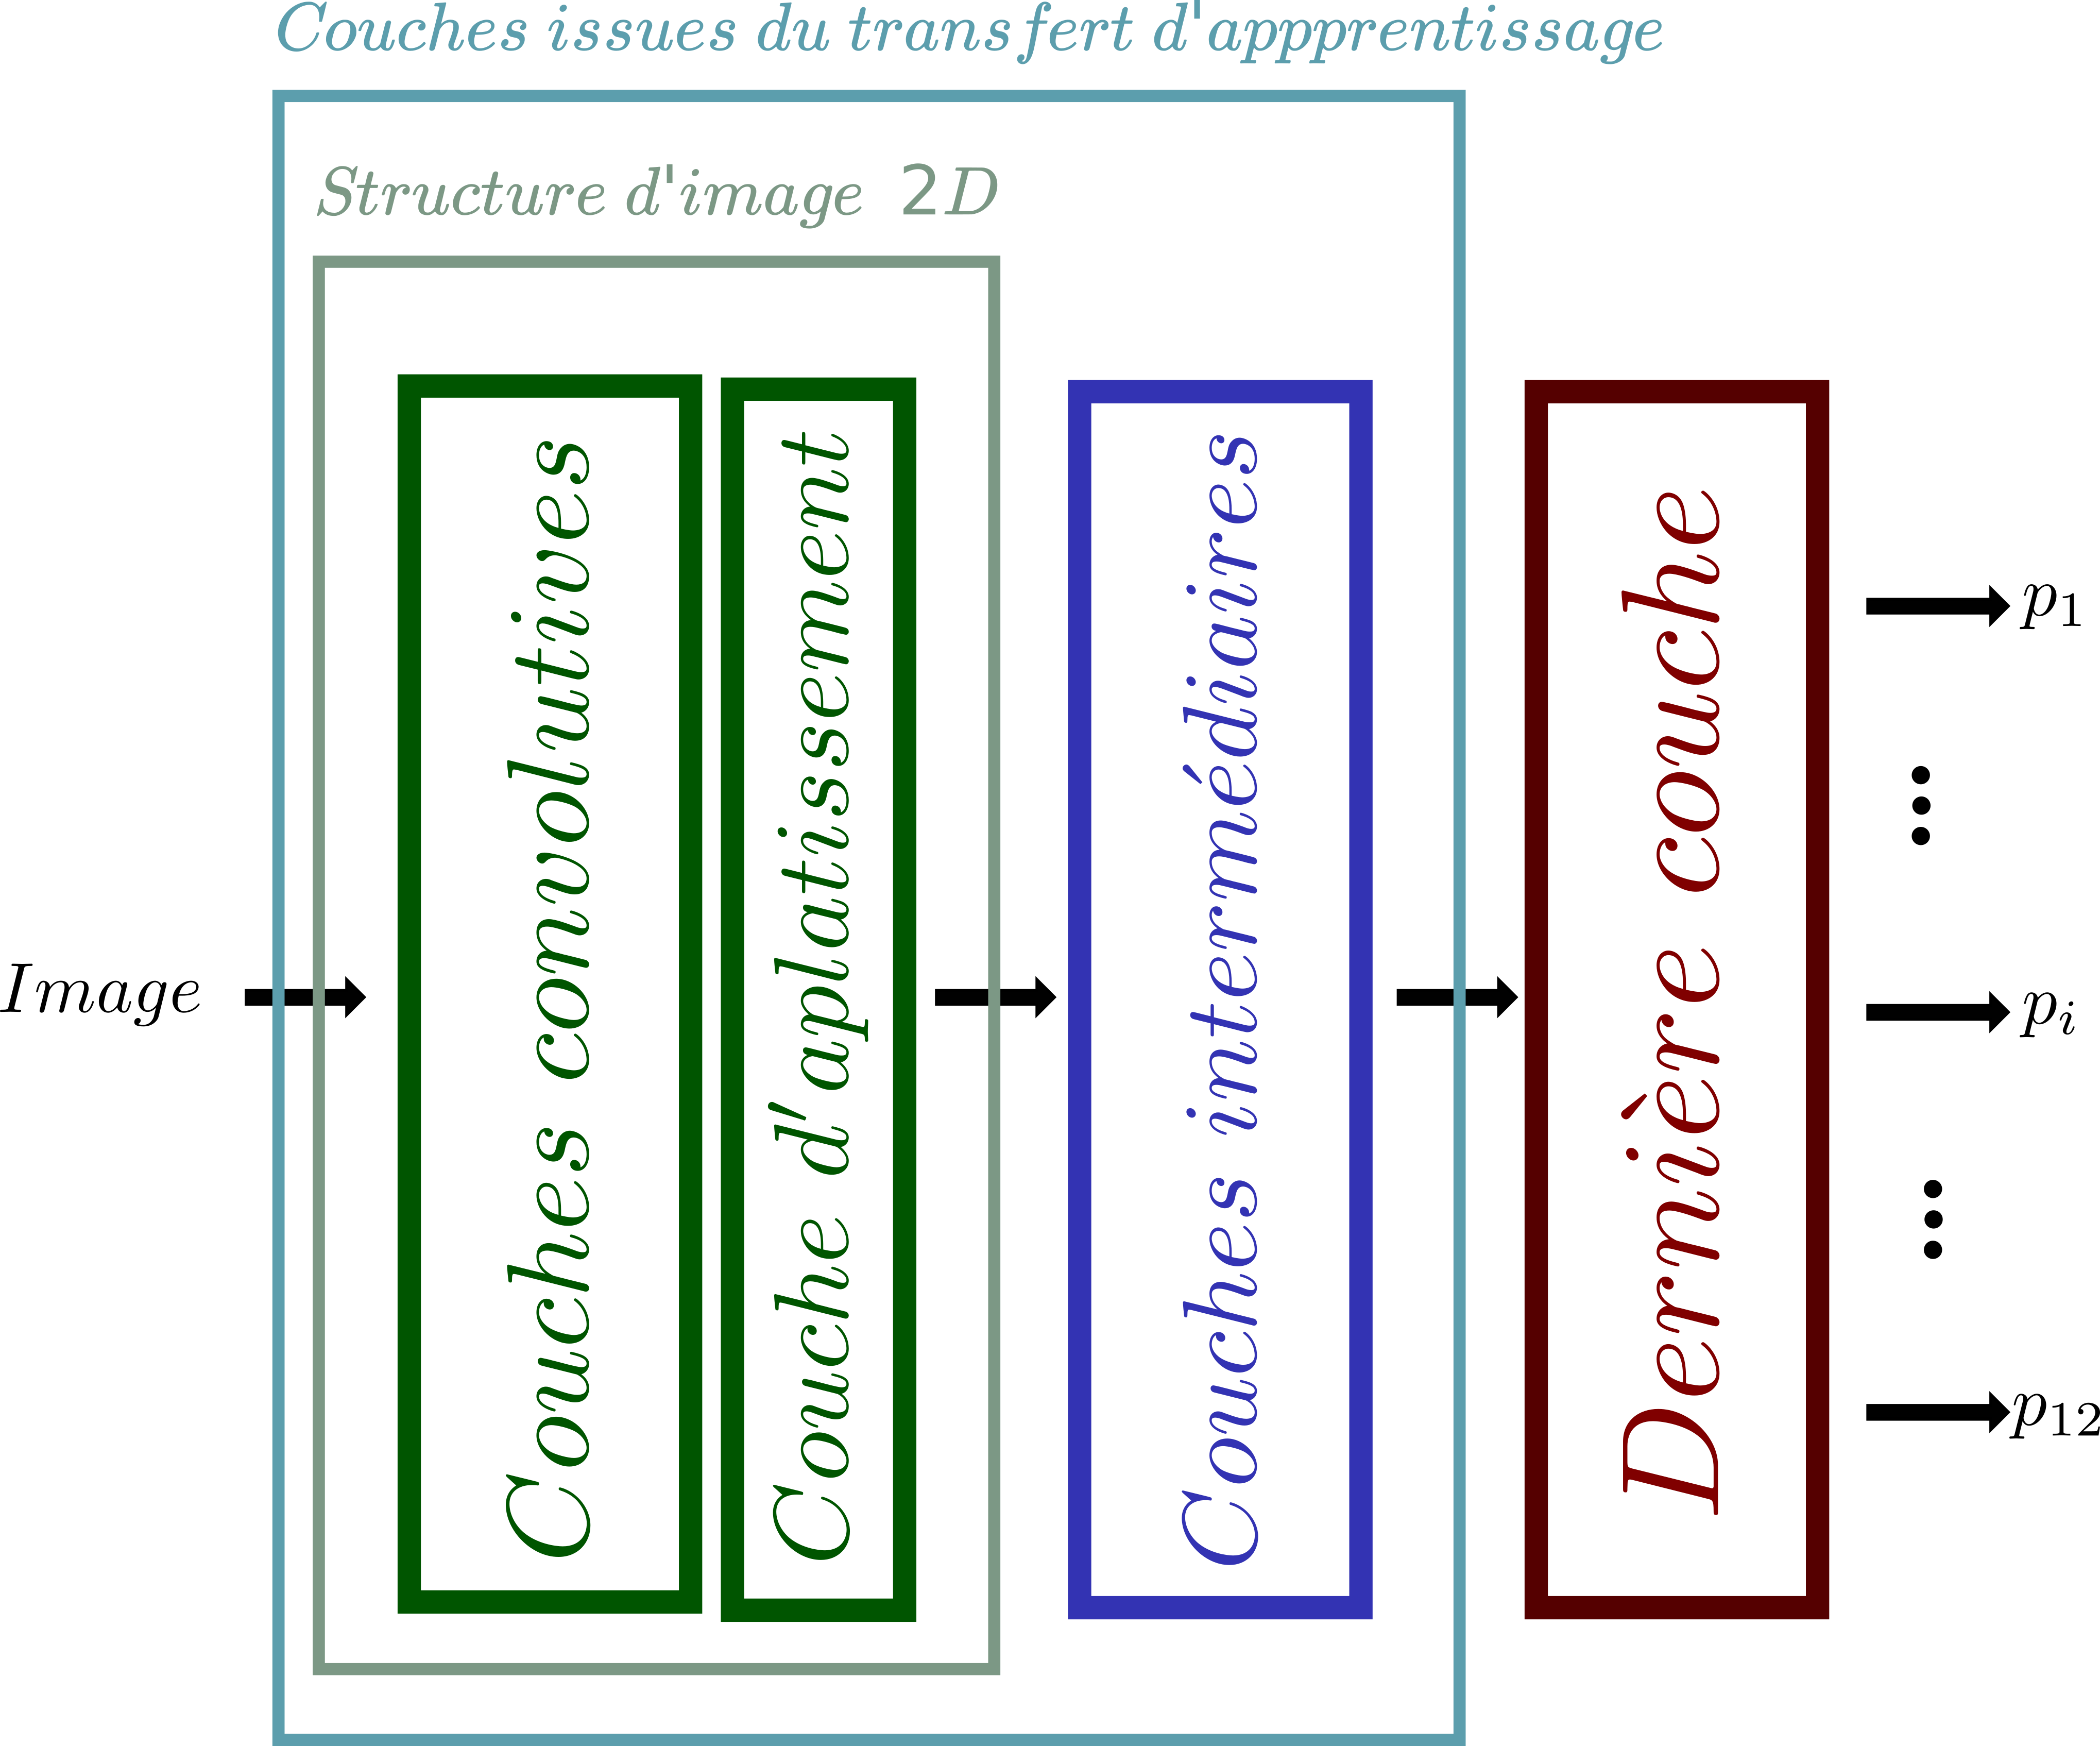
\includegraphics[height=0.8\textheight]{6-schema.png}
		\caption{Structure de mon réseau de neurones}
	\end{figure}
	

\end{frame}